\section{Theoretische Grundlagen}
\label{sec:theoretische_grundlagen}
Atome können in verschiedene Energieniveaus angeregt werden. Dabei werden
Elektronen aus ihrem Grundzustand in einen Zustand höherer Energie gebracht.
Die niedrigsten Niveaus werden dabei als S- und P-Schalten bezeichnet.  Das
Verhältnis der Besetzungszahlen $N_1$ und $N_2$ dieser Zustände ohne äußeres
Magnetfeld wird dabei durch die Boltzmann-Verteilung beschrieben:
\begin{equation}
\label{eq:boltzmann}
    \frac{N_2}{N_1} = \frac{g_2}{g_1}\cdot
        \mathrm{e}^\frac{W_1 - W_2}{k_\text{B}T}\,.
\end{equation}
Dabei bezeichnet $g_i$ und $W_i$ ein jeweiliges statistisches Gewicht,
beziehungsweise die jeweilige Energie $T$ die Temperatur und $k_\text{B}$ die
bekannte Boltzmann-Konstante.

Diese Verteilung kann durch optisches Pumpen beeinflusst werden.
Durch Einstrahlung von Licht der Wellenlänge
\begin{equation}
\label{eq:wellenlaenge}
    h\nu = W_2 - W_1
\end{equation}
können Übergänge vom niedrigeren Energieniveau $W_1$ in das höhere Niveau
$W_2$ angeregt werden. Außerdem können Elektronen spontan oder induziert in ein
niedrigeres Niveau fallen, wobei ein neues Quant der Energie
\ref{eq:wellenlaenge} abgestrahlt wird.

\subsection{Zeeman-Effekt und Hyperfeinstruktur}
\label{subsec:zeemanneffekt_und_hyperfeinstruktur}
Die Energiestruktur von Atomen ist unter anderem durch den Gesamtdrehimpuls
$\vec{L}$ und Spin $\vec{S}$ der Elektronenhülle, sowie den Kernspin $\vec{I}$
bestimmt. Dabei sind mit diesen Drehimpulsen die magnetischen Momente
\begin{align}
    \vec{\mu}_L &= -\mu_\text{B}\vec{L}\,,
        \label{eq:magn_moment_elektronen}\\
    \vec{\mu}_S &= -g_S\mu_\text{B}\vec{S}\,,
        \label{eq:magn_moment_espin}\\
    \text{und}\qquad\vec{\mu}_I &= -g_I\mu_\text{B}\vec{I}
        \label{eq:magn_moment_kernspin}
\end{align}
verknüpft, wobei $g_I$ und $g_S$ die Landé-Faktoren bezeichnen und
$\mu_\text{B}$ das Bohrsche Magneton.
Der Gesamtdrehimpuls der Elektronenhülle koppelt dabei an den Kernspin,
was zur sogenannten Hyperfeinstruktur führt.
Zusätzlich kann der gesamte Drehimpuls $\vec{F} = \vec{J} + \vec{I}$ an äußere
magnetische Felder koppeln, was zu einer weiteren Aufspaltung in $\num{2}F +
\num{1}$ Niveaus für jedes Niveau der Hyperfeinstruktur führt.
Dieser Effekt ist in Abbildung \ref{fig:aufspaltung} schematisch dargestellt.
\begin{figure}
    \centering
    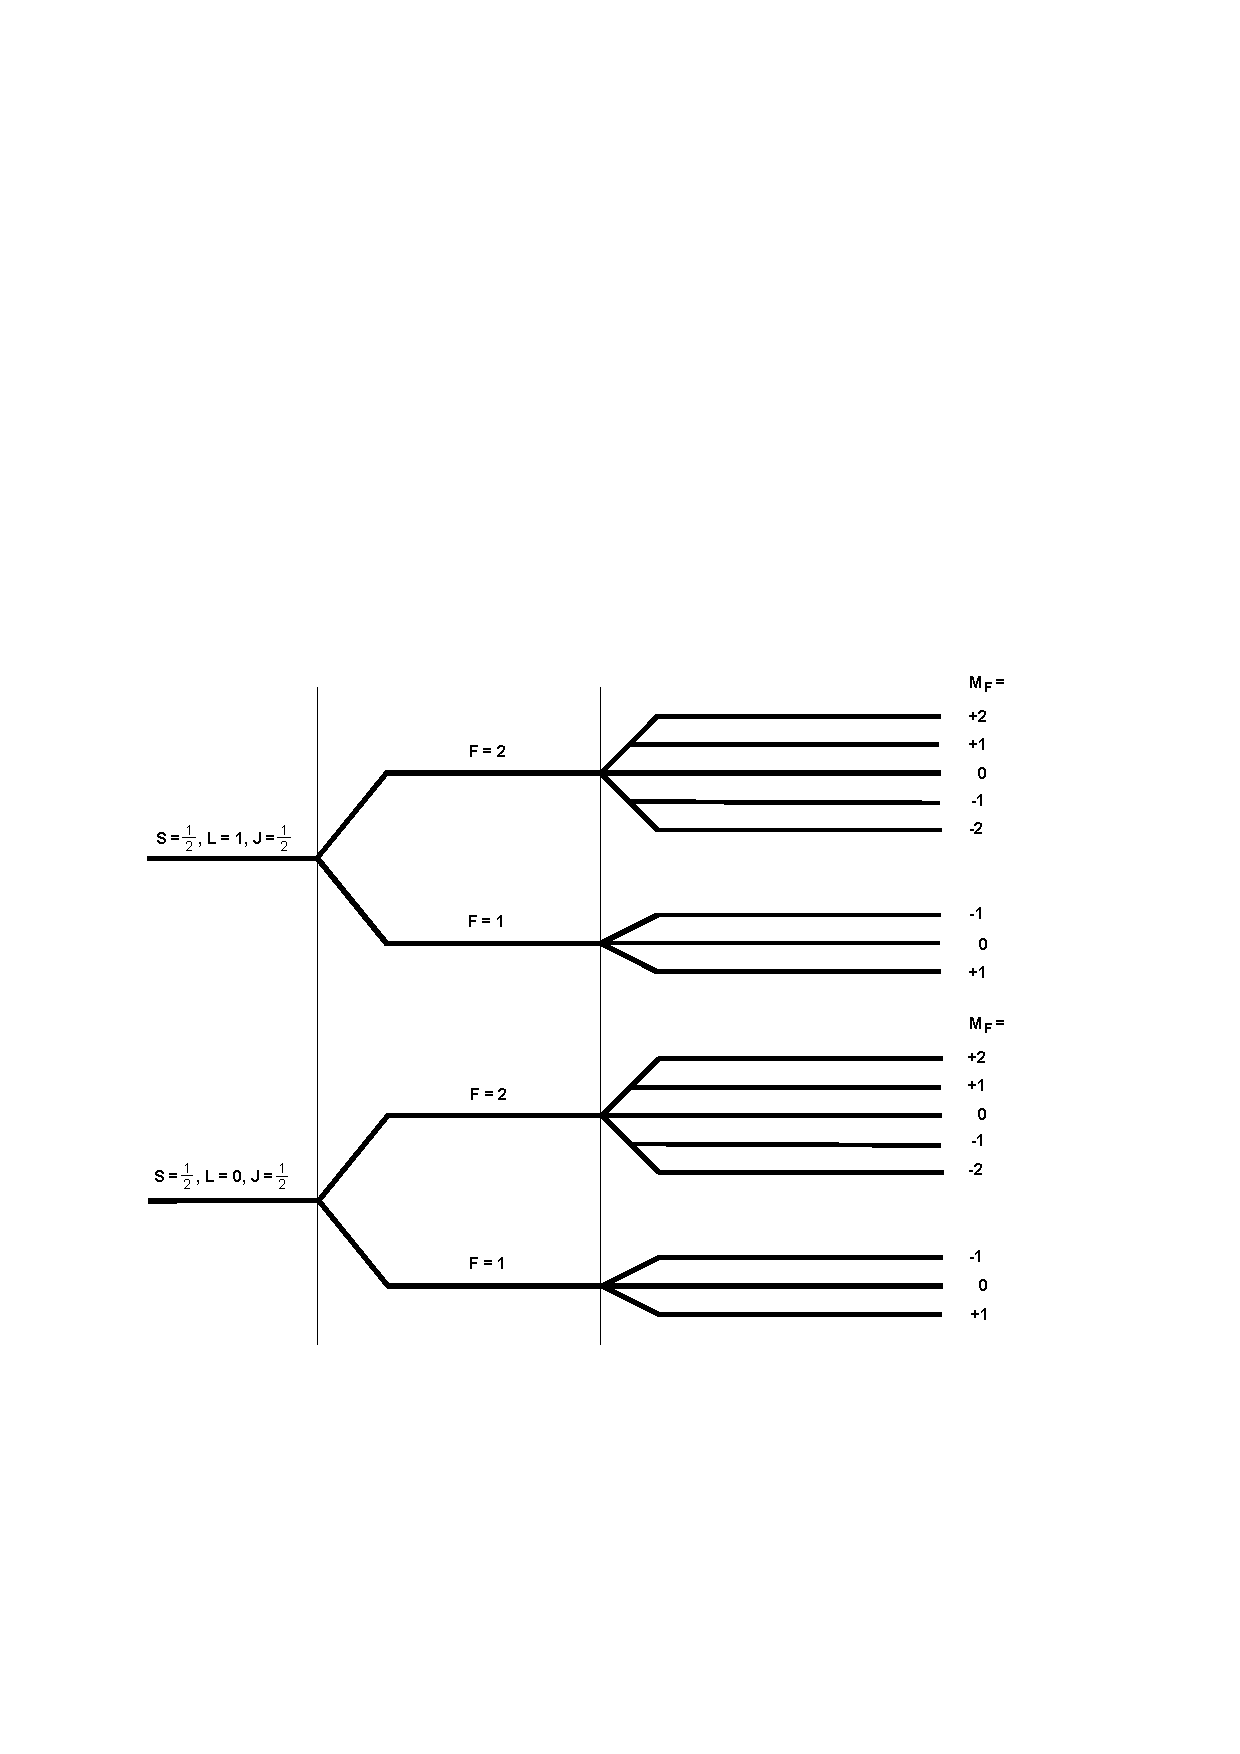
\includegraphics[width=0.8\linewidth]{img/aufspaltung.pdf}
    \caption{
        Energieaufspaltung eines Alkali-Atoms mit Kernspin $I=\sfrac{3}{2}$
        \cite{V21}.
    }
    \label{fig:aufspaltung}
\end{figure}
Die Energie benachbarter Zeeman-Niveaus unterscheidet sich dabei jeweils um
\begin{equation}
\label{eq:zeeman_energie}
    U_\text{HF} = g_F \mu_\text{B} B\,,
\end{equation}
mit dem Landé-Faktor $g_F$ und einem äußeren Magnetfeld der Feldstärke $B$.
Aus der vektoriellen Betrachtung der magnetischen Momente und deren Richtungsquantelung folgt für den Landé-Faktor des Atoms
\begin{equation}
\label{eq:lande_faktor}
    g_F = g_J \frac{F(F+1) + J(J+1) - I(I+1)}{2F(F+1)}\,.
\end{equation}
Da $g_S$ bekannt ist, kann zudem $g_J$ bestimmt werden zu
\begin{equation}
\label{eq:gj}
    g_J = \frac{\num{3.0023}\cdot J(J+1)
                + \num{1.0023}\cdot\left[S(S+1) - L(L+1)\right]}
               {2J(J+1)}
          \,.
\end{equation}

\subsection{Optisches Pumpen}
\label{subsec:optisches_pumpen}

